%% This is the fee-thesis example file. It is used to produce theses
%% for submission to the Faculty of electrical engineering, University of West Bohemia
%%
%% Get the newest version from
%% https://gitlab.ket.zcu.cz/templates/feethesis-latex
%%
%% Copyright 2022, Jan Belohoubek
%%
%% This work may be distributed and/or modified under the
%% conditions of the LaTeX Project Public Licenese, either version 1.3
%% of this license or (at your option) any later version.
%% The latest version of this license is in
%%  https://www.latex-project.org/lppl.txt
%% and version 1.3 or later is part of all distributions of LaTeX
%% version 2005/12/01 or later.
%%
%% This work has the LPPL maintenance status `maintained'.
%%
%% The current maintainer of this work is Jan Belohoubek (belohoub@fel.zcu.cz).
%% Please, submit bug reports into the tracker at
%% https://gitlab.ket.zcu.cz/templates/feethesis-latex/-/issues
%%
%% This work was derived from the FIT CTU Theses template
%% by Eliska Sestakova and Ondrej Guth (ce1138a0474df18ba5add79f3373a216afba0098)
%%
%% The FIT CTU template can be obtained from:
%% https://gitlab.fit.cvut.cz/theses-templates/FITthesis-LaTeX


%%%%%%%%%%%%%%%%%%%%%%%%%%%%%%%%%%%%%%%%%
% CLASS OPTIONS
% language: czech/english/slovak
% thesis type: bachelor/master/dissertation
%%%%%%%%%%%%%%%%%%%%%%%%%%%%%%%%%%%%%%%%%
\documentclass[czech,bachelor,unicode,12pt]{fee-thesis}

%%%%%%%%%%%%%%%%%%%%%%%%%%%%%%%%%%
% FILL IN THIS INFORMATION
%%%%%%%%%%%%%%%%%%%%%%%%%%%%%%%%%%
\feetitle{Kryptografický akcelerátor s SPI interfacem} % replace with the title of your thesis
\feeauthorfull{Libor Miller} % replace with your full name (first name(s) and then family name(s) / surname(s)) including academic degrees
\feeauthorgivennames{Libor} % replace with your first name(s) / given name(s)
\feeauthorsurnames{Miller} % replace with your surname(s) / family name(s)
\feesupervisor{doc. Ing. Martin Poupa, Ph.D.} % replace with name of your supervisor/advisor (include academic degrees)
\feedepartment{Katedra elektroniky a informačních technologií} % replace with the department of your defence
\feeyear{2027} % replace with the year of your defence
\feedeclarationplace{Plzni} % replace with the place where you sign the declaration
\feedeclarationdate{\today} % replace with the date of signature of the declaration

% CS HELP ===================================================== % 
% Abstrakt představuje stručný výtah ze závěrečné práce (miniatura práce) a umožňuje čtenáři prvotní, velmi rychlou, orientaci v dané práci, slouží k vytvoření představy o jejím obsahu. Abstrakt by měl obsahovat stručný popis podstaty řešení uvedeného v závěrečné práci, dále by měly být zmíněny použité metody řešení, díky nimž bylo daného řešení dosaženo. Měly by být také uvedeny dosažené výsledky a odpovídající závěr. Abstrakt v daném jazyce by svým rozsahem neměl překročit jednu stranu, obvykle je jeho délka 80 až 500 slov (tj. minimálně 6 řádků). Abstrakt se uvádí jak v češtině, tak v angličtině.
% ============================================================= %

\feeabstractCZE{Práce se zabývá implementací kryptografického jádra SIMON s SPI slave rozhraním do integrovaného obvodu vyrobeného technologií SKY130A. Celý proces návrhu se tedy dá rozdělit na dvě části, digitální a analogovou. Veškerá digitální logika je realizována pomocí jazyku Verilog, z čehož byla pomocí LibreLane syntetizována část návrhu integrovaného obvodu. Tato digitální část byla testována na několika úrovních. Logický test kódu pomocí simulátoru Icarus Verilog, který byl ovládán auotmatizačním Python scriptem. Stejný test pak byl aplikován na netlist logických bran vytvořený syntézou, ale hlavní validací byl funkční test na FPGA s reálným SPI masterem. Další část návrhu byla vytvořena pomocí EDA nástrojů XSCHEM a Magic. Touto medodou byl vytvořen kruhový oscilátor s nastavitelnou frekvencí, který slouží jako interní hodinový zdroj.}

\feeabstractENG{This thesis deals with the implementation of the SIMON cryptographic core with an SPI slave interface, into an integrated circuit manufactured using SKY130A technology. The entire design process can therefore be divided into two parts: digital and analogue. All the digital logic is implemented using the Verilog language, from which part of the integrated circuit design was synthesised using LibreLane. This digital section was tested at several levels. Test od logic using the Icarus Verilog simulator, which was controlled by an automation Python script. The same test was then applied to the netlist of logic gates generated by synthesis, however, the main validation was a functional test on an FPGA with a real SPI master. Another part of the design was created using the EDA tools XSCHEM and Magic. Using this method, a frequency-adjustable ring oscillator was created, which serves as an internal clock source.}

% CS HELP ===================================================== % 
% Klíčová slova jsou konkrétní fráze reprezentující řešenou problematiku. Klíčová slova se uvádějí na stejnou stranu společně s abstraktem v češtině a angličtině. Klíčová slova se řadí od obecných pojmů ke konkrétním.
% ============================================================= % 

\feekeywordsCZE{kryptografie, SPI, ASIC, Verilog}
\feekeywordsENG{cryptography, SPI, ASIC, Verilog}

%%%%%%%%%%%%%%%%%%%%%%%%%%%%%%%%%%
% END FILL IN
%%%%%%%%%%%%%%%%%%%%%%%%%%%%%%%%%%

%%%%%%%%%%%%%%%%%%%%%%%%%%%%%%%%%%
% CUSTOMIZATION of this template
% Skip this part or alter it if you know what you are doing.
%%%%%%%%%%%%%%%%%%%%%%%%%%%%%%%%%%

\RequirePackage{iftex}[2020/03/06]
\iftutex % XeLaTeX and LuaLaTeX
    \RequirePackage{ellipsis}[2020/05/22] %ellipsis workaround for XeLaTeX
\else
    \RequirePackage[utf8]{inputenc}[2018/08/11] %this file encoding
    \RequirePackage{lmodern}[2009/10/30] % vector flavor of Computer Modern font
\fi

% show hyperlinks
%\RequirePackage[pdfpagelayout=TwoPageRight,colorlinks=false,allcolors=decoration,pdfborder={0 0 0.1}]{hyperref}[2020-05-15]

% hide hyperlinks
\RequirePackage[pdfpagelayout=TwoPageRight,hidelinks]{hyperref}[2020-05-15]

\RequirePackage{pdfpages}[2020/01/28]

\setcounter{secnumdepth}{4} % numbering sections; 4: subsubsection

% Default ToC depths
\addtocontents{lot}{\protect\setcounter{tocdepth}{1}}%
\addtocontents{lof}{\protect\setcounter{tocdepth}{1}}%
\addtocontents{app}{\protect\setcounter{tocdepth}{1}}
\addtocontents{toc}{\protect\setcounter{tocdepth}{3}}%

%%%%%%%%%%%%%%%%%%%%%%%%%%%%%%%%%%
% CUSTOMIZATION of this template END
%%%%%%%%%%%%%%%%%%%%%%%%%%%%%%%%%%

%%%%%%%%%%%%%%%%%%%%%%
% DEMO CONTENTS SETTINGS
% You may choose to modify this part.
%%%%%%%%%%%%%%%%%%%%%%
\usepackage{dirtree}
\usepackage{lipsum,tikz, circuitikz}
\usepackage{csquotes}
\usepackage[style=iso-numeric]{biblatex}
\addbibresource{text/bib-database.bib}
\usepackage{listings} % typesetting of sources
\usepackage{float}
% \usepackage{minted} % typesetting of sources

%theorems, definitions, etc.
\theoremstyle{plain}
\newtheorem{theorem}{Věta}
\newtheorem{lemma}[theorem]{Tvrzení}
\newtheorem{corollary}[theorem]{Důsledek}
\newtheorem{proposition}[theorem]{Návrh}
\newtheorem{definition}[theorem]{Definice}
\theoremstyle{definition}
\newtheorem{example}[theorem]{Příklad}
\theoremstyle{remark}
\newtheorem{note}[theorem]{Poznámka}
\newtheorem*{note*}{Poznámka}
\newtheorem{remark}[theorem]{Pozorování}
\newtheorem*{remark*}{Pozorování}
\numberwithin{theorem}{chapter}
%theorems, definitions, etc. END
%%%%%%%%%%%%%%%%%%%%%%
% DEMO CONTENTS SETTINGS END
%%%%%%%%%%%%%%%%%%%%%%

% FEE template currently recomends no indentions of the paragraphs
\parindent=0pt

\begin{document} 
\frontmatter\frontmatterinit % do not remove these two commands

\thispagestyle{empty}\cleardoublepage\maketitle % do not remove these three commands

% set speciffic spacing
\setstretch{1.5}



\printabstractpage % do not remove this command

%%%%%%%%%%%%%%%%%%%
% ACKNOWLEDGMENT
% FILL IN / MODIFY / COMMENT
% This is a place to thank people for helping you. It is common to thank your supervisor.
%%%%%%%%%%%%%%%%%%%

% CS HELP ===================================================== % 
% Student zde vyjádří míru spolupráce se zadávající katedrou, případně dalšími pracovišti v průběhu vypracovávání kvalifikační práce a má možnost poděkovat zde vedoucímu práce, případně konzultantovi a dalším. Poděkování je \textbf{nepovinnou částí kvalifikační práce.}
% ============================================================= %

\begin{acknowledgmentpage}
  Chtěl bych poděkovat svému vedoucímu za podporu. Také bych chtěl poděkovat projektu Tiny Tapeout, bez kterého by výroba integrovaného obvodu nebyla možná.
\end{acknowledgmentpage} 
%%%%%%%%%%%%%%%%%%%
% ACKNOWLEDGMENT END
%%%%%%%%%%%%%%%%%%%

%%%%%%%%%%%%%%%%%%%%%%
% Table of contents BEGIN
%%%%%%%%%%%%%%%%%%%%%%

\clearpage

% CS HELP ===================================================== % 
% Obsah práce
% Zařazen na začátku práce, stránky s obsahem se nečíslují. Každá položka obsahu by se měla vejít na jeden řádek. Čísla stránek v obsahu se zarovnávají k pravému kraji stránky. Čísla stránek v obsahu udávají číslo první stránky, na níž začíná příslušná kapitola nebo subkapitola. Na stránce s obsahem není žádný jiný text.
% ============================================================= %

\tableofcontents % do not remove this command

\clearpage

%%%%%%%%%%%%%%%%%%%%%%
% Table of contents END
%%%%%%%%%%%%%%%%%%%%%%

% CS HELP ===================================================== % 
% Seznam symbolů a zkratek
% Seznam symbolů a zkratek je abecedně seřazen, přičemž proměnné a konstanty zapsané pomocí znaků řecké abecedy jsou řazeny až na konci seznamu; někdy bývá zvykem zkratky abecedně seřadit samostatně a odděleně až za symboly, proměnnými a konstantami.
% ============================================================= %
\chapter*{Seznam symbolů}

\section*{Obecné}

\begin{tabular}{p{4.4cm} l}
$I$ & skalární veličina \\
$\underline{I}$ & fázor skalární veličiny \\
$A$ & vektorová veličina \\
$\underline{A}$ & fázor vektorové veličiny \\
$A_Z$ & složka vektorové veličiny \\
\end{tabular}

\section*{Magnetické a proudové pole}

\begin{tabular}{p{2cm} p{2cm} l}
$I$ & A & elektrický proud \\
$B$ & B & magetická indukce \\
$H$ & A/m & intenzita magnetického pole \\
\end{tabular}

\section*{Elektrické pole}

\begin{tabular}{p{2cm} p{2cm} l}
$Q$ & C & elektrický náboj \\
$D$ & C/m$^2$ & elektrická indukce \\
$E$ & V/m & intenzita elektrického pole \\
\end{tabular}

\section*{Teplotní pole}

\begin{tabular}{p{2cm} p{2cm} l}
$T$ & K & teplota \\
$F$ & W/m$^2$ & hustota tepelného toku \\
$G$ & K/m & teplotní gradient \\
\end{tabular}

\chapter*{Seznam zkratek}
	
\begin{tabular}{p{4cm} l}
LWC & Light weigth cryptography\\
TT & Tiny Tapeout \\
FPGA & Field-programmable gate array \\
ASIC & Application-specific integrated circuit \\
MWP & Multi-wafer project
\end{tabular}

%%%%%%%%%%%%%%%%%%%
% ABBREVIATIONS END
%%%%%%%%%%%%%%%%%%%

\mainmatter\mainmatterinit % do not remove these two commands

%%%%%%%%%%%%%%%%%%%
% THE TEXT BEGIN
%
% include other files if necessary
%%%%%%%%%%%%%%%%%%%

% Do not forget to include Introduction
%---------------------------------------------------------------
% \chapter{Introduction}
% uncomment the following line to create an unnumbered chapter
\chapter*{Úvod}\addcontentsline{toc}{chapter}{Úvod}\markboth{Úvod}{Úvod} % \markboth is used due to page footer
%---------------------------------------------------------------
\setcounter{page}{1}

% CS HELP ===================================================== % 
% Úvod obsahuje, čím se práce zabývá, jaký problém je v práci řešen a jeho jasnou definici. Dále je zde uvedeno, proč je dané téma řešeno (tj. důvod vzniku zadání) a nastíněn postup řešení. Tato část obsahuje shrnutí současných možných zjištěných řešení jiných autorů. Může také obsahovat popis myšlenek, které byly aplikovány jinými autory při řešení stejného nebo podobného problému. Jsou zde také hojně uvedeny komentované bibliografické citace informačních zdrojů, ze kterých bylo při rešerši čerpáno.
%
% Úvod rozhodně nepředstavuje nepodstatnou část kvalifikační práce, do které autor uvede zcela bezvýznamný text s cílem zaplnění této části tak, aby nezůstala zcela prázdná. Úvod také neslouží k laickému popisu problematiky řešené v kvalifikační práci, protože tato je odbornou prací, kde jsou předpokládány určité odborné znalosti čtenáře. V úvodu by měl být diskutovány následující body.
%% - Zdůvodnění aktuálnosti tématu a nastínění problému, který student bude řešit.
%% - Stanovení cíle (cílů) práce.
%% - Vytvoření hlavních otázek, na které chce práce najít odpověď.
%% - Nastínění použitých metod a struktury práce.
%
% Úvod práce typicky neobsahuje číslované sekce, speciální prostředí, vzorce, apod.
% ============================================================= % 


V roce 2025 bylo k síti připojeno 21.1 biliónů IoT zařízení \cite{connected_devices} a každým rokem toto číslo roste
o 10 až 15\%. Podle zprávy bezpečnostní agentury Palo Alto \cite{Unit2020} z roku 2020 až 57\% IoT zařízení nemá žádnou nebo nedostačující formu
zabezpečení. Tato zařízení jsou tak pro útočníky jednoduchý vstupní bod do sítě. Krom obav z ransomwareu je na místě také
strach z intercepce datových zpráv, protože většina jich není nijak zašifrovaná a putují skrz síť pouze jako enkodovaný text.

Tato práce se zabývá jedním z cenově a energeticky nenáročných řešení. Tím je hardwareová implementace LWC v podobě externího crypto-chipu, konkrétně šifry SIMON v konfiguraci
s 64 bitovým klíčem a 32 bitovým blokem šifrovaných dat. Tato konfigurace je kompromis mezi úrovní zabezpečení a počtem logických bran ze kterých se skládá.
Oproti běžně používaným standardům jako je AES128, je realizace této šifry prostorově i energreticky mnohem úspornější \cite{Diehl2017} a je tak vhodná
i pro kooperacei s 8 a 16 bitovými kontrolery s extrémně nízkou spotřebou. Návrh, o kterém pojednává tato práce, má krom samotné šifry i sběrnici SPI a nastavitelný generátor interního hodinového signálu.

%---------------------------------------------------------------
\chapter{Workflow a využité nástroje}\label{chap:main}
%---------------------------------------------------------------
Většina nástrojů, které byly k realizaci projektu použity, jsou open-source. Jedinou výjimkou je IDE Intel Quartus, které bylo použito pro práci s FPGA. Využitím opensource nástrojů v kombinaci s projektem Tiny Tapeout \cite{Venn2024} bylo možné snížit výrobní cenu prototypu integrovaného obvodu z několika desítek až stovek tisíc USD na 550 USD.
Tato radikální redukce ceny vyplývá zejména z vyhnutí se programům s komerční licencí. Další faktor pro redukci ceny byl výběr vhodné výrobní technologie. Nejedná se o zařízení, které by potřebovalo nejmodernější výrobní procesy. Dostačují 130 nm technologie IHPSG13G2, na které byl založený první prototyp a SKY130A, na které byl založený druhý prototyp. Důvodem pro změnu technologií byl rozdíl datumů, kdy se uzavírala výrobní okna.
Vzhledem k tomu, že první prototyp obsahuje jen digitální část, která zůstala stejná i pro druhý, bude se pojednávat jen o druhém prototypu a technologii SKY130A. Narozdíl od výroby standardních několikavrstvých PCB, které se dají dnes nechat vyrobit za poměrně nízké ceny s lhůtou dodání v rámci dní až týdnů, je výroba prototypů integrovaných obvodů mnohem nákladnější a zdlouhavější. 
Výroba integrovaného obvodu s sebou obnáší obrovské jednorázové fixní náklady, zejména kvůli výrobě fotolitografických masek, které se pro každý nový design mění. Tyto masky se pak dají použít k výrobě velkých sérií, kde se náklady na kus rozloží. U prototypů však nedává smysl vyrábět velké série a jednorázové náklady se musí rozložit jen na pár desítek až stovek kusů. Kvůli komplexním dodavatelským řetězcům a aktuálnímu přetížení většiny výrobců polovodičů výrobní lhůty trvají několik měsíců, během kterých mohou nastat mnohá neplánovaná zpoždění. Z toho důvodu je nutné klást důraz na simulace a prototyp se nechává vyrábět až v okamžiku, kdy je design kompletně verifikován a existuje vysoká pravděpodobnost toho, že bude fungovat. 

\section{Tiny Tapeout}
Jak bylo nastíněno výše, výroba prototypů integrovaného obvodu je komplexní, zdlouhavý a drahý proces. Z cenových důvodů bylo možné návrh na reálný silikon implementovat jen jediným aktuálně (2026) dostupným způsobem, a to skrze Tiny Tapeout. 
Princip Tiny Tapeout je jednoduchý, zkompiluje přibližně 500 projektů a umístí je do jediného integrovaného obvodu. Pomocí páteřního multiplexoru se vybírá aktivní projekt,který je propojený s definovanými pady pouzdra. Každý projekt je power gated a je napájen jen tehdy, když je aktivně vybrán. Aby se design mohl stát součástí sdíleného výrobního cyklu, musí splňovat pravidla a projít několika testy. Tím se zabrání tomu, aby jeden nekorektní projekt znehodnotil celý ASIC. 
Tiny Tapeout neodesílá finální ASIC přímo do polovodičové továrny, ale do MPW. V závislosti na výrobní technologii se mění využitý MPW. Znamená to tedy že projekt odeslaný do TT je na sdíleném chipu, který se vyrobí na sdíleném waferu, ze kterého se vyrobí minimálně 20 různých integrovaných obvodů \cite{Venn2024,chipfoundry_howitworks} . Díky této struktuře je možné dosáhnout nízké ceny a pro malé projekty je velikost použitelného prostoru na chipu dostačující.
\section{Výrobní technologie SKY130A}
SKY130A je jedna z mála technologií pro výrobu pokročilých integrovaných obvodů, která má opensource PDK. Z toho plyne několik zásadních výhod: žádné poplatky za využití technologie, nižší ceny výroby, žádné smlouvy o mlčenlivosti a také mnohé komunitní projekty, 
díky kterým je možné technologii reálně využít \cite{skywater_sky130A}.\newline
PDK obsahuje několik má částí, které umožňují návrh obvodů \cite{STG2020}.
\begin{itemize}
  \item DRC pravidla, pro návrh. Definují minimální velikosti vodičů, substrátů, a jiných vrstev.
  \item Knihovna standardních součástek. V té jsou obsažené tranzistory, hradla, klopné obvody, multiplexory a další primitivní struktury.
  \item SPICE modely pro veškeré standartní struktury.
  \item Popisy fyzikálních vlastností materiálů.
  \item Pravidla pro LVS. Ta umožňují porovnat schéma s layoutem.
\end{itemize}

\begin{figure}[H]
  \centering
  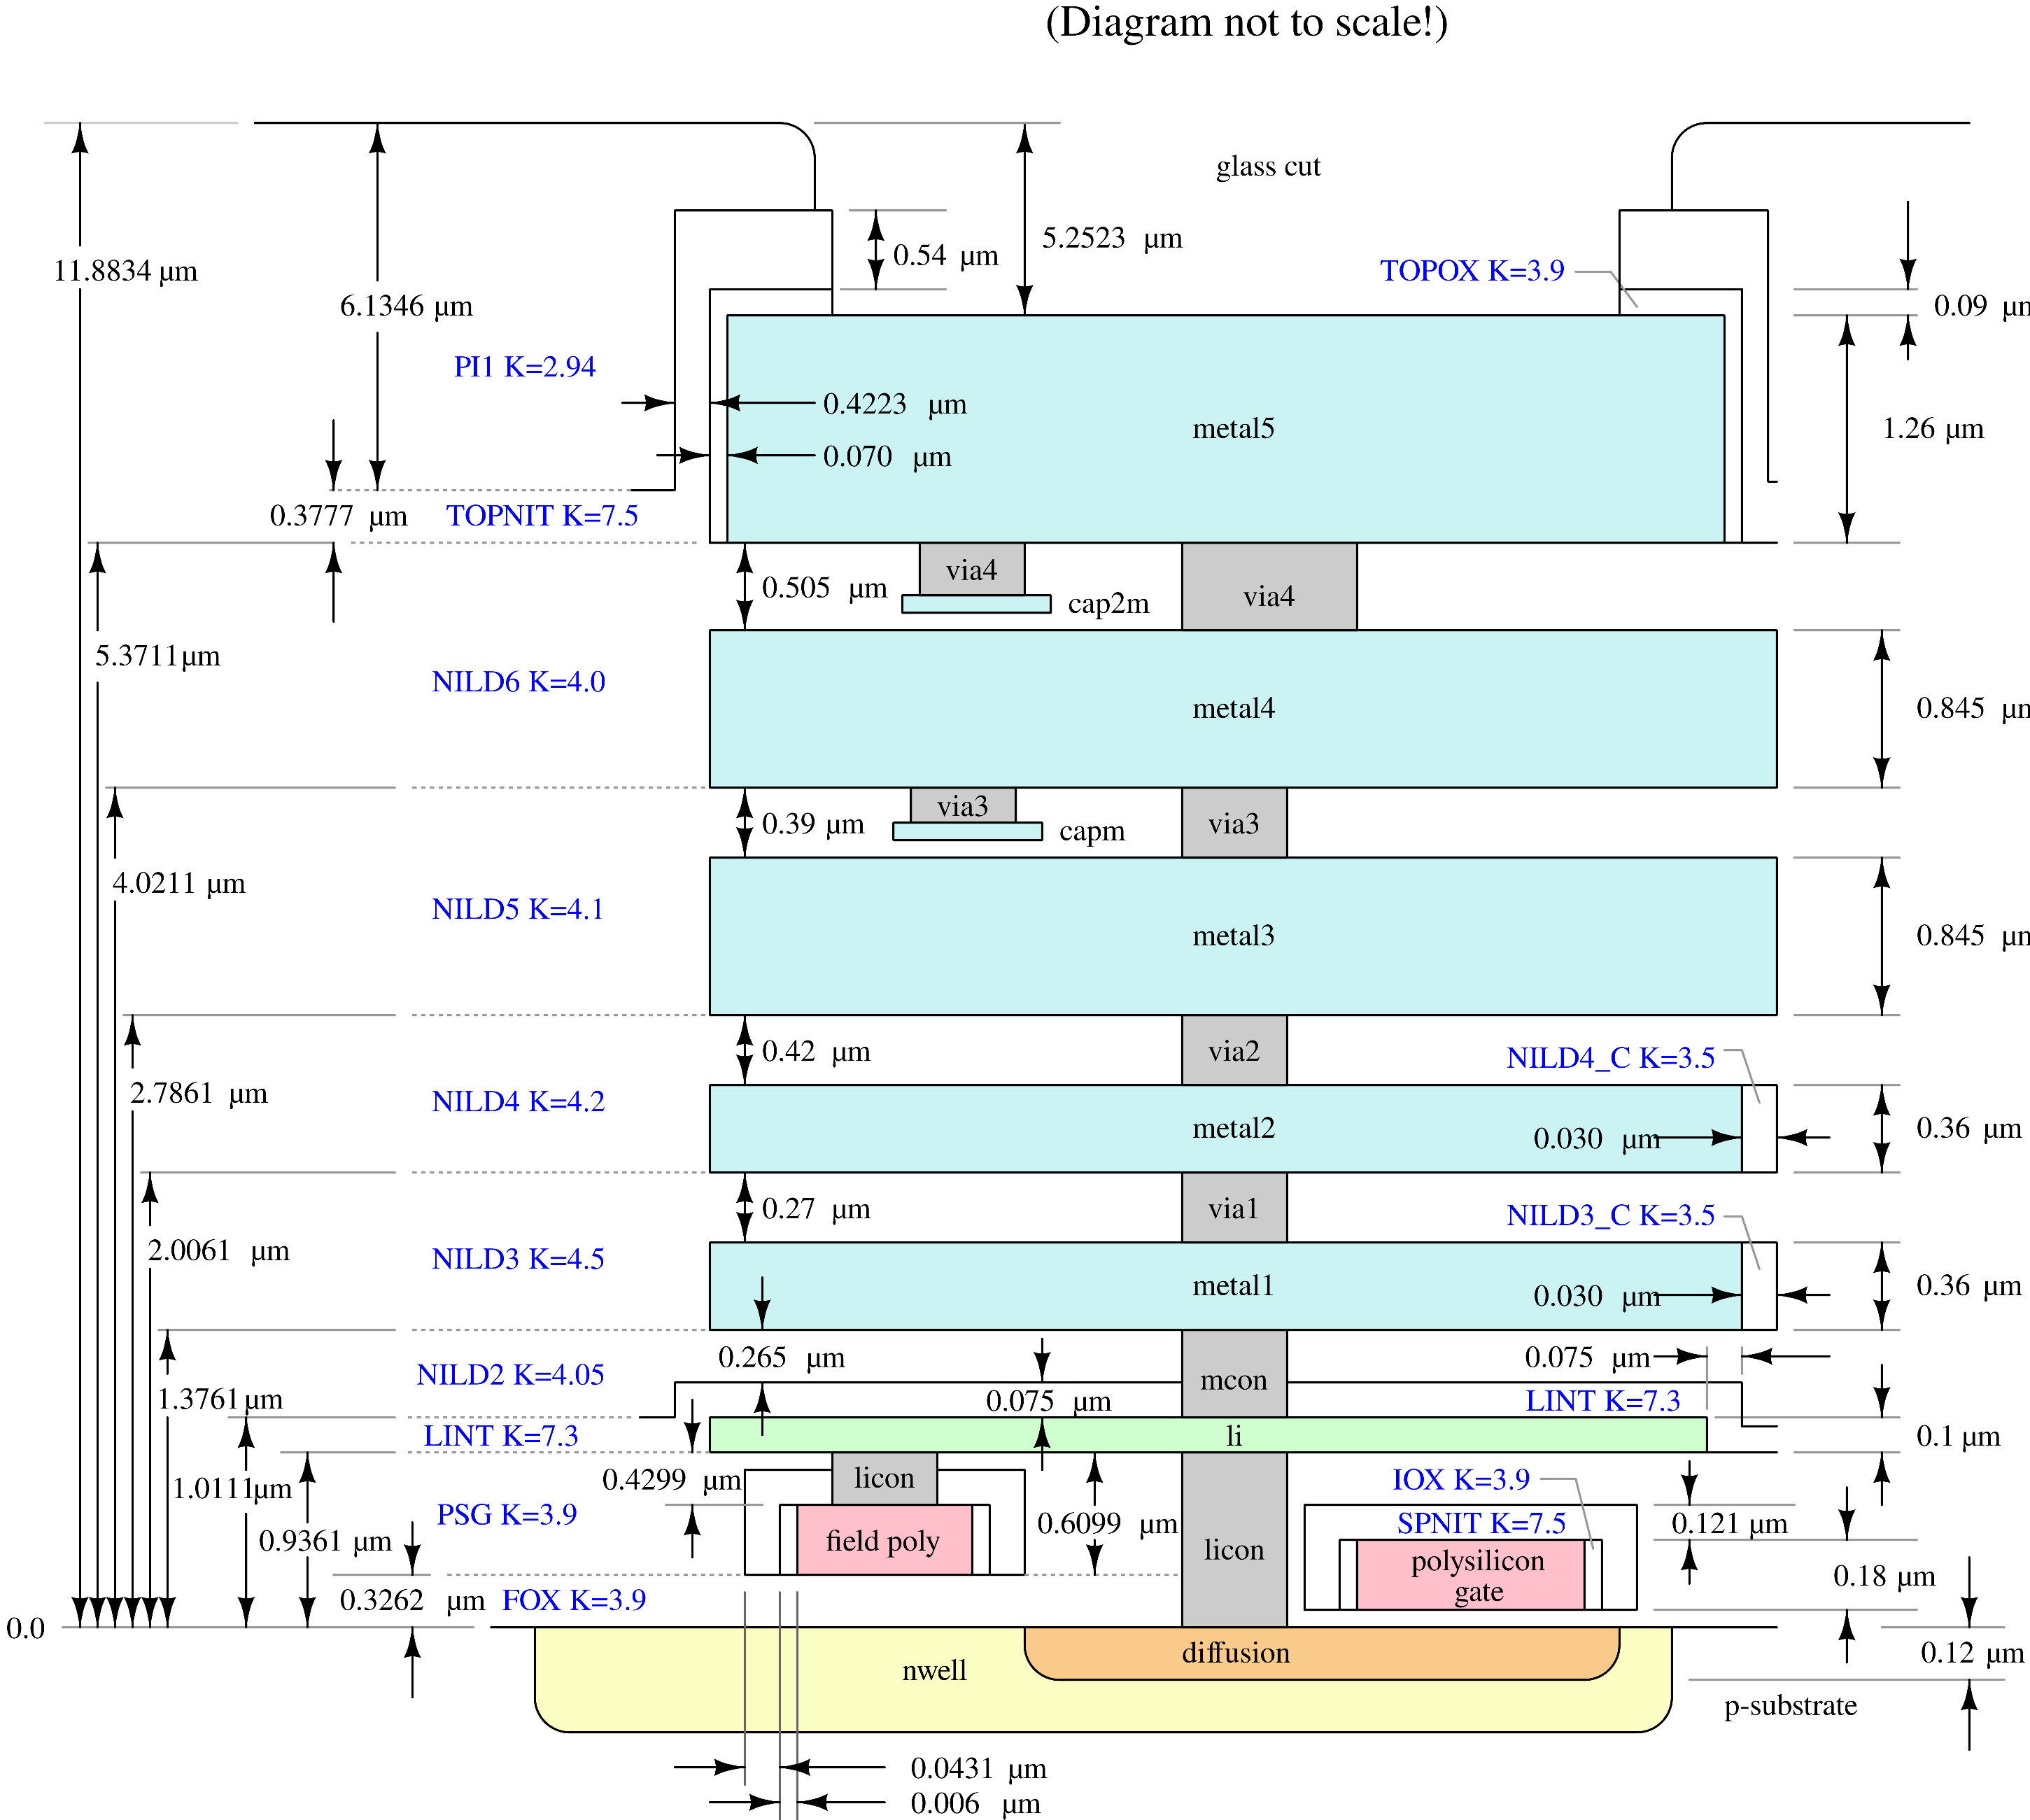
\includegraphics[scale=0.25]{img/metal_stack.pdf}
  \caption{Průřez vrstvami které je možné vytvořit procesem SKY130A \cite{skywater_metal_stack}.}\label{img:metal_stack}
\end{figure}

V tomto procesu je podkladový substrát typu P. V tomto substrátu je možné vytvářet struktury typu N a hloubkové N studny. Proces je optimalizován pro tvorbu unipolárních tranzistorů,
ale umožňuje i bipolární tranzistory. Cesty se dají vést na 6 vrstvách kovu a Tiny Tapeout si nejvyšší vrstvu vyhrazuje pro rozvod napájení. Je možné vytvořit kondenzátory i rezistory.
Vzhledem k fyzickým rozměrům lze vytvářet jen kondenzátory o maximální kapacitě desítek fF a to několika způsoby, v této práci se využívají dva, buď se vytvoří mosfet a propojí se source s drainem a využívá se jeho kapacita
na gate, výhoda je relativně velká kapacita, ale za cenu nelinearity ($C=f(U)$), druhou možností je využít speciální vrstvy \textit{cap2m}, nebo \textit{capm}, které dovolí vytvořit kondenzátor mezi dvěma kovovými ploškami,
tento způsob je vhodný pro přesné,malé a lineární kapacity. Absolutní hodnoty rezistorů se silně liší s každým výrobním během, proto je vhodnější využívat poměry odporů, namísto absolutních hodnot. Realizace cívek na chipu je 
prakticky téměř nevyužitelná \cite{skywater_sky130A,jku_analog,cmos_analog_design}.

\section{Proces návrhu integrovaného obvodu}
Jedna z nevýhod využívání opensource nástrojů je jejich roztříštěnost. Neexistuje tedy jeden centrální program, ve kterém by se dalo udělat vše od verilogu po layout a floorplanning. Je tedy nutné se zorientovat 
v relativně velkém množství komplexních nástrojů vyvýjených malými týmy či jednotlivci. Souhrn a popis všech nástrojů v Tabulce \ref{tab:nastroje_ic_design}.
\begin{table}[!ht]
    \centering
    \caption[Nástroje využívané pro návrh integrovaných obvodů]{Nástroje využívané pro návrh integrovaných obvodů}\label{tab:nastroje_ic_design}
    \begin{tabular}{|l|l|}
    \hline
        \textbf{Nástroj} & \textbf{Popis} \\ \hline
        Verilog & HDL sloužící k popisu logických obvodů. \\ \hline
        Verilator & Logický simulátor pro verilog. \\ \hline
        Intel Quartus & Vývojové prostředí pro FPGA Intel .\\ \hline
        Librelane & Syntetizátor Verilog kódu do fyzického obvodového zapojení ve formátu GDS. \\ \hline
        XSCHEM & Editor elektronických schémat. \\ \hline
        NGSPICE & Simulátor SPICE. \\ \hline
        Magic & Layout editor pro integrované obvody. \\ \hline
        Klayout & Alternativní layout editor pro integrované obvody. \\ \hline
        Netgen & Porovnává zapojení layoutu a schématu. \\ \hline
        SKY130A PDK & Soubor nástrojů a výrobních pravidel pro proces SKY130A. \\ \hline
    \end{tabular}
\end{table}

Proces návrhu se liší pro digitální a analogovou část. Digitální část je založená na HDL Verilogu, který je automaticky syntetizován do podoby logických hradel ze standardní knihovny. Proces syntézy obstarává program LibreLane.
U analogové části projektu bylo nutné vytvořit ručně schéma i layout nejen ze standardních komponent PDK, ale i vlastních součástek.
Celý proces je znázorněn pracovním diagramem na Obrázek \ref{fig:design_diag}.

\begin{figure}[H]
\centering
\resizebox{0.6\textwidth}{!}{%
\begin{circuitikz}
\tikzstyle{every node}=[font=\fontsize{11.9pt}{15.5pt}\selectfont]
\draw  (11.125,11.125) rectangle (14,12.5);
\node[anchor=center, align=center, inner xsep=0.080cm, inner ysep=0.085cm, rounded corners=0.020cm, font=\fontsize{11.9pt}{15.5pt}\selectfont] at (12.5625,11.8125) {XSCHEM};
\draw  (11.125,12.875) rectangle (14,14.25);
\node[anchor=center, align=center, inner xsep=0.080cm, inner ysep=0.085cm, rounded corners=0.020cm, font=\fontsize{11.9pt}{15.5pt}\selectfont] at (12.5625,13.5625) {NGSPICE};
\draw  (11.125,14.625) rectangle (14,16);
\node[anchor=center, align=center, inner xsep=0.080cm, inner ysep=0.085cm, rounded corners=0.020cm, font=\fontsize{11.9pt}{15.5pt}\selectfont] at (12.5625,15.3125) {Magic/Klayout};
\draw  (11.125,16.375) rectangle (14,17.75);
\node[anchor=center, align=center, inner xsep=0.080cm, inner ysep=0.085cm, rounded corners=0.020cm, font=\fontsize{11.9pt}{15.5pt}\selectfont] at (12.5625,17.0625) {Netgen};
\draw  (11.125,18.125) rectangle (14,19.5);
\node[anchor=center, align=center, inner xsep=0.080cm, inner ysep=0.085cm, rounded corners=0.020cm, font=\fontsize{11.9pt}{15.5pt}\selectfont] at (12.5625,18.8125) {Post layout \\ NGSPICE};
\draw  (19.25,9.375) rectangle (22.125,10.75);
\node[anchor=center, align=center, inner xsep=0.080cm, inner ysep=0.085cm, rounded corners=0.020cm, font=\fontsize{11.9pt}{15.5pt}\selectfont] at (20.6875,10.0625) {Verilog};
\draw  (19.25,12.875) rectangle (22.125,14.25);
\node[anchor=center, align=center, inner xsep=0.080cm, inner ysep=0.085cm, rounded corners=0.020cm, font=\fontsize{11.9pt}{15.5pt}\selectfont] at (20.6875,13.5625) {FPGA \\ verifikace};
\draw  (19.25,14.625) rectangle (22.125,16);
\node[anchor=center, align=center, inner xsep=0.080cm, inner ysep=0.085cm, rounded corners=0.020cm, font=\fontsize{11.9pt}{15.5pt}\selectfont] at (20.6875,15.3125) {LibreLane};
\draw  (19.25,16.375) rectangle (22.125,17.75);
\node[anchor=center, align=center, inner xsep=0.080cm, inner ysep=0.085cm, rounded corners=0.020cm, font=\fontsize{11.9pt}{15.5pt}\selectfont] at (20.6875,17.0625) {Gate level \\ Verilator};
\draw  (19.25,18.125) rectangle (22.125,19.5);
\node[anchor=center, align=center, inner xsep=0.080cm, inner ysep=0.085cm, rounded corners=0.020cm, font=\fontsize{11.9pt}{15.5pt}\selectfont] at (20.6875,18.8125) {GDS, LEF};
\draw  (19.25,11.125) rectangle (22.125,12.5);
\node[anchor=center, align=center, inner xsep=0.080cm, inner ysep=0.085cm, rounded corners=0.020cm, font=\fontsize{11.9pt}{15.5pt}\selectfont] at (20.6875,11.8125) {Verilator};
\draw  (15.25,18.125) rectangle (18.125,19.5);
\node[anchor=center, align=center, inner xsep=0.080cm, inner ysep=0.085cm, rounded corners=0.020cm, font=\fontsize{11.9pt}{15.5pt}\selectfont] at (16.6875,18.8125) {.def \\ template};
\draw  (13.75,19.875) rectangle (19.375,22.75);
\node[anchor=center, align=center, inner xsep=0.080cm, inner ysep=0.085cm, rounded corners=0.020cm, font=\fontsize{11.9pt}{15.5pt}\selectfont] at (16.5625,21.3125) {Vrcholová integrace v \\ XSCHEMU};
\draw  (15.125,23.125) rectangle (18,24.5);
\node[anchor=center, align=center, inner xsep=0.080cm, inner ysep=0.085cm, rounded corners=0.020cm, font=\fontsize{11.9pt}{15.5pt}\selectfont] at (16.5625,23.8125) {Magic/Klayout};
\draw  (15.125,24.875) rectangle (18,26.25);
\node[anchor=center, align=center, inner xsep=0.080cm, inner ysep=0.085cm, rounded corners=0.020cm, font=\fontsize{11.9pt}{15.5pt}\selectfont] at (16.5625,25.5625) {Netgen};
\draw [-{Stealth[scale=1.5]}, ] (12.5,14.25) -- (12.5,14.625);
\draw [-{Stealth[scale=1.5]}, ] (12.5,12.5) -- (12.5,12.875);
\draw [-{Stealth[scale=1.5]}, ] (12.5,16) -- (12.5,16.375);
\draw [-{Stealth[scale=1.5]}, ] (12.5,17.75) -- (12.5,18.125);
\draw [-{Stealth[scale=1.5]}, ] (20.625,10.75) -- (20.625,11.125);
\draw [-{Stealth[scale=1.5]}, ] (20.625,12.5) -- (20.625,12.875);
\draw [-{Stealth[scale=1.5]}, ] (20.625,14.25) -- (20.625,14.625);
\draw [-{Stealth[scale=1.5]}, ] (20.625,16) -- (20.625,16.375);
\draw [-{Stealth[scale=1.5]}, ] (20.625,17.75) -- (20.625,18.125);
\draw [short] (12.5,19.5) -- (12.5,20.875);
\draw [short] (20.625,19.5) -- (20.625,20.875);
\draw [-{Stealth[scale=1.5]}, ] (12.5,20.875) -- (13.75,20.875);
\draw [-{Stealth[scale=1.5]}, ] (20.625,20.875) -- (19.375,20.875);
\draw [-{Stealth[scale=1.5]}, ] (16.75,19.5) -- (16.75,19.875);
\draw [-{Stealth[scale=1.5]}, ] (16.625,22.75) -- (16.625,23.125);
\draw [-{Stealth[scale=1.5]}, ] (16.625,24.5) -- (16.625,24.875);
\draw [short] (11,13.625) -- (9.5,13.625);
\draw [short] (9.5,13.625) -- (9.5,11.625);
\draw [short] (11.125,13.625) -- (10.875,13.625);
\draw [-{Stealth[scale=1.5]}, ] (9.5,11.625) -- (11.125,11.625);
\draw [short] (11.125,17.125) -- (9.5,17.125);
\draw [short] (9.5,17.125) -- (9.5,15.5);
\draw [-{Stealth[scale=1.5]}, ] (9.5,15.5) -- (11.125,15.5);
\draw [short] (11.125,18.75) -- (8.625,18.75);
\draw [short] (8.625,18.75) -- (8.625,11.375);
\draw [-{Stealth[scale=1.5]}, ] (8.625,11.375) -- (11.125,11.375);
\draw [short] (22.125,11.875) -- (23.5,11.875);
\draw [short] (23.5,11.875) -- (23.5,10.25);
\draw [-{Stealth[scale=1.5]}, ] (23.5,10.25) -- (22.125,10.25);
\draw [short] (22.125,13.75) -- (23.875,13.75);
\draw [short] (23.875,13.75) -- (23.875,10);
\draw [-{Stealth[scale=1.5]}, ] (23.875,10) -- (22.125,10);
\draw [short] (22.125,17.125) -- (24.25,17.125);
\draw [short] (24.25,17.125) -- (24.25,9.75);
\draw [-{Stealth[scale=1.5]}, ] (24.25,9.75) -- (22.125,9.75);
\draw [short] (15.125,25.625) -- (14,25.625);
\draw [short] (14,25.625) -- (14,23.75);
\draw [-{Stealth[scale=1.5]}, ] (14,23.75) -- (15.125,23.75);
\draw  (15.125,26.625) rectangle (18,28);
\node[anchor=center, align=center, inner xsep=0.080cm, inner ysep=0.085cm, rounded corners=0.020cm, font=\fontsize{11.9pt}{15.5pt}\selectfont] at (16.5625,27.3125) {GDS, LEF};
\draw [-{Stealth[scale=1.5]}, ] (16.625,26.25) -- (16.625,26.625);
\end{circuitikz}
}%
\caption{Diagram procesu návrhu a verifikace integrovaného obvodu.}
\label{fig:design_diag}
\end{figure}

\subsection{Analogové workflow}
Základem vytváření analogových částí jsou programy XSCHEM, Magic, Klayout, NGSPICE a Netgen. V XSCHEMu se vytvoří schéma a na základě definovaných parametrů součástek se vygeneruje SPICE netlist celého schématu. Díky čemuž je možné vytvořit podrobnou simulaci a ověřit funkci obvodu z ideálních součástek.
SPICE netlist se dá naimportovat do Magicu, který slouží k vytvoření layoutu. Generátor vytvoří fyzické součástky dle definovaných parametrů v netlistu. Je možné generátor nevyužít, ale znamenalo by to, že je nutné vytvořit každý tranzistor, rezistor i kondenzátor z elementárních materiálů jako je P substrát a N substrát.
Během vytváření layoutu Magic kontroluje DRC živě a přepočítává je na mřížce 0.1 $\mu m$, což znamená že některé chyby se nemusí projevit a je nutné nechat design projít kontrolou DRC i v programu Klayout, který je přesnější. Pro zjištění zda-li layout odpovídá schématu je nutné využít nástroj Netgen,
který porovnává SPICE netlist vygenerovaný programy XSCHEM a Magic. Po vytvoření fyzického zapojení je dobré vyextrahovat parazitní kapacity i sériové odpory a zvalidovat návrh stejným SPICE testem, kterým bylo testováno schématické zapojení.
Vzhledem k tomu že layout je po jeho vytvoření neflexibilní. Je vhodné postupovat hierarchicky a modulárně, tzn. vytvořit menší blok zvalidovat ho a začlenit do vyššího celku.

\subsection{Digiální workflow}

% CS HELP ===================================================== % 
% V~následujícím textu je popsána metodika zpracování VŠKP. Hlavní text je vhodné rozčlenit následujícím způsobem.
%
% Teoretická (metodologická) část
% Obsahuje dosavadní poznatky k~danému problému, definici pojmů, formulaci hypotéz, výběr použitých metod a~důvody pro jejich použití, součástí teoretické části bývá i~rozbor možných variant řešení.
%
%
% Kvalifikační práce
% Bakalářskou prací student prokazuje, že je schopen řešit a~ústně i~písemně prezentovat zadaný problém a~obhájit své vlastní přístupy k~řešení. Obsah bakalářské práce odpovídá charakteru daného studijního oboru. Obsahem bakalářské práce mohou zpravidla být:
% - odborná zpráva na základě rešerše, vycházející z~teoretických poznatků získaných studiem odborné literatury, ve které student přehledně shrnuje již známé skutečnosti, hodnotí je a~vyvozuje vlastní závěry v~dané problematice,
% - odborná zpráva, vycházející z~vlastních nebo převzatých experimentálních výsledků, která obsahuje zpracování získaných dat vhodnými metodami a~vyvození závěrů,
% - výpočet a~návrh jednoduššího technického zařízení nebo jeho části, zpracovaný na základě poznatků získaných v~průběhu studia a~studiem literatury, dokumentovaný postupem a~popisem výpočtu, vypracováním technické dokumentace zařízení, popř. i~zhotovením jeho funkčního vzorku,
% - odborná zpráva, obsahující technickoekonomický rozbor několika variant řešení téhož problému.
%
% Diplomovou prací student prokazuje, že je schopen řešit a~ústně i~písemně prezentovat zadaný problém a~obhájit své vlastní přístupy k~řešení.  Předpokládá se uplatnění invence studenta, prezentace jeho vlastního pohledu na řešenou problematiku. Obsah diplomové práce odpovídá charakteru daného studijního oboru. Diplomová práce se liší od bakalářské práce zejména charakterem zadaných problémů, rozsahem a~hloubkou jejich zpracování a~přínosem vlastních poznatků. Obsahem diplomové práce mohou zpravidla být:
% - odborná zpráva, vycházející z~vlastních experimentálních výsledků, která obsahuje zpracování získaných dat vhodnými metodami a~vyvození závěrů,
% - výpočet a~návrh složitějšího technického zařízení nebo jeho části, zpracovaný na základě poznatků získaných v~průběhu studia a~studiem literatury, dokumentovaný postupem a~popisem výpočtu, vypracováním technické dokumentace zařízení, popř. i~zhotovením jeho funkčního vzorku,
% - odborná zpráva, obsahující technickoekonomický rozbor několika variant řešení téhož přiměřeně náročného problému.
%
% Kvalifikační práce je vizitkou autora, proto vedle náležité obsahové úrovně by měla mít i~odpovídající formální strukturu a~úpravu. Rozsah kvalifikační práce je specifikován v~zadání, doporučený rozsah hlavní textové části bakalářské práce je obvykle 30 až 40 normostran, doporučený rozsah hlavní textové části diplomové práce je 40 až 60 normostran, kde jedna normostrana odpovídá textu o~délce 1800 znaků.
%
% Při psaní kvalifikační práce je nutno dbát na srozumitelnost textu a~logickou návaznost jednotlivých kapitol. Zcela zásadní je zřetelné oddělení výsledků vlastní práce od výsledků převzatých od jiných autorů. Veškerou použitou literaturu je nutno důsledně citovat podle ČSN ISO 690 Bibliografické odkazy a~citace dokumentů. Nezbytné je dodržení gramatických pravidel.
%
% V~souladu s~etickou normou je zakázáno opisování nebo kopírování souvislých pasáží z~publikací jiných autorů bez uvedení (citace) zdroje. Takové jednání je posuzováno jako neoprávněné přivlastňování si cizích myšlenek a~může vést k~hodnocení známkou „nevyhověl“, v~závažnějších případech i~ke kárnému řízení. (Všechny kvalifikační práce jsou po odevzdání testovány na plagiátorství v~systému Theses.cz).
%
% Pro zpracování kvalifikační práce platí doporučení normy ČSN 01 6910 Úprava dokumentů zpracovaných textovými procesory.
%
% Autor a~vedoucí práce si primárně stanoví pravidla vzájemné komunikace a~způsobu konzultací (termíny, frekvence, forma), které jsou pro studenta závazné.
%
%
% Praktická (tvůrčí) část
% Obsahuje řešení problému, experimenty, výpočty, diskusi a~vyhodnocení přínosu práce. Představuje tvůrčí část práce.
%
% Ve vlastních kapitolách práce autor popisuje detailní rozbor stavu problému, navrhuje a~definuje postup řešení/použité metody řešení, popisuje vlastní řešení a~jeho verifikaci (ověření věrohodnosti výsledků), popisuje praktickou realizaci experimentů/měření/ oživování zařízení atd.
%
% Popis experimentálních metod/měření musí být proveden tak, aby bylo možné experiment opakovat. Musí být zdůvodněno použití zvolených metod. Zvolené metody musí umožňovat vhodnou interpretaci dat (nesmí zkreslovat výsledky). Autor také nesmí opomenout uvést popis statistického zpracování výsledků případných použitých měřicích metod.
%
% Výsledky měření/výpočtů by měly být nejdříve jasně uvedeny a~následně je možné provést jejich diskusi, vyhodnocení a~interpretaci.
%
% V~kvalifikační práci je doporučeno popsat všechna řešení, a~to i~ta, která nevedla k~cíli a~napomohla např. k~jeho nalezení, případně vyloučila některé nevhodné způsoby řešení.
%
% Jednotlivé kapitoly by měly být vhodně logicky rozčleněny a~každá by měla začínat na nové stránce. Názvy kapitol, oddílů a~pododdílů se nesmí v~celé práci měnit.
% ============================================================= % 


%---------------------------------------------------------------
\chapter{Struktura a použití šablony}\label{chap:struct}
%---------------------------------------------------------------

Šablona pro tvorbu závěrečné práce na FEL ZČU ve formátu \LaTeX{} má následující strukturu:

\dirtree{%
    .1 ~.
    .1 img\DTcomment{adresář s obrázky}.
    .1 text\DTcomment{adresář se zdrojovými texty}.
    .2 appendix.tex\DTcomment{přílohy práce ve formátu \LaTeX{}}.
    .2 assignment-include.pdf\DTcomment{zadání práce}.
    .2 medium.tex\DTcomment{obsah přiloženého média ve formátu \LaTeX{}}.
    .2 text.tex\DTcomment{text práce ve formátu \LaTeX{}}.
    .2 bib-database.bib\DTcomment{bibliografická databáze ve formátu BibTeX}.
    .1 fee-thesis.cls\DTcomment{šablona \LaTeX{}u}.
    .1 fee-thesis.tex\DTcomment{hlavní zdrojový soubor práce ve formátu \LaTeX{}}.
    .1 LICENSE\DTcomment{licence šablony}.
    .1 README.md\DTcomment{popis projektu a základní nápověda}.
}

\bigskip

\begin{note}
  Kódování zdrojových souborů \LaTeX{}u je \texttt{UTF-8}.
\end{note}

\begin{note}
Typ práce zvolíte změnou deklarace v hlavičce dokumentu \texttt{fee-thesis.tex}: zvolte bakalářskou nebo diplomovou práci.
\end{note}

\bigskip

Ve většině případů v souboru \texttt{fee-thesis.tex} pouze vyplníte základní údaje o práci jako je název práce, jméno autora a vedoucího, název katedry obhajoby, abstrakt a seznam klíčových slov a seznamy symbolů a zkratek.

Vlastní text práce pak tvoříte v samostatných souborech v adresáři \texttt{text}. V souboru \texttt{text/text.tex} se nachází hlavní část textu práce, soubor \texttt{text/appendix.tex} obsahuje přílohy a soubor \texttt{text/medium.tex} je určen pro popis obsahu elektronické přílohy práce.

Soubor \texttt{text/bib-database.bib} obsahuje databázi citací ve formátu BibTeX -- do databáze vložte záznamy pro materiály, které budete v práci citovat.

Soubor \texttt{assignment-include.pdf} nahraďte naskenovaným zadáním práce.

\bigskip

\begin{note}
  v souboru \texttt{fee-thesis.tex} můžete odstranit blok \texttt{acknowledgmentpage}, nechcete-li do práce zahrnout poděkování.
\end{note}

%---------------------------------------------------------------
\chapter{Práce se šablonou}
%---------------------------------------------------------------

Tato šablona definuje základní styly dokumentu dle pokynů pro vypracování závěrečných prací na FEL ZČU.

Níže jsou uvedeny příklady použití direktiv \LaTeX{}u v souladu s aktuálními pokyny pro vypracování závěrečných prací na FEL. 

% CS HELP ===================================================== % 
% Formátování textu
% Stanovuje základní pravidla pro samotný text a jeho grafickou úpravu v celé práci, kdy cílem je dosáhnout jednotného stylu formátování, tak aby práce byla graficky přehledná a kompaktní. V obsahu se projeví pouze první tři úrovně nadpisů, tedy je vhodné používat pouze Nadpis 1 – 3. Pro stať práce je doporučen styl „Normální“. 
%% - Práce jsou psány pro formát A4, řádkování 1,5.
%% - Odsazení levého okraje stránky 3 cm.
%% - Odsazení zbylých okrajů stránky 2,5 cm.
%% - Používá se jeden základní typ písma: Times New Roman.
%% - Velikost písma 10 – názvy tabulek, grafů, obrázků a legendy či zdroje k nim, poznámky pod čarou
%% - Velikost písma 12 – standardní text práce, nadpisy podkapitol
%% - Velikost písma 16 – hlavní nadpisy
%% - Text je možné zvýrazňovat kurzívou, tučným písmem či podtržením (pokud je zdůrazňován víceslovný výraz, podtrhává se nepřetržitě).
%% - Text se zarovnává do bloku, nadpisy vlevo.
%% - Číslování textu práce začíná od první strany úvodu a končí poslední stránkou závěru.
%% - Záhlaví obsahuje název práce, jméno autora, rok zpracování.
%% - Zápatí obsahuje čísla stránek.
%
% Členění textu
% Kapitoly začínají na novém listu papíru. Nadpisy se uvádějí na samostatných řádcích a nepíše se za nimi tečka. Členění obsáhlejšího textu se provádí titulky a podtitulky, píší se malými písmeny kromě velkých začátečních písmen.
% Na konci stránky nesmí zůstat nadpis kapitoly, samotná první řádka odstavce a slovo ukončené rozdělovacím znaménkem. % Na začátek stránky nesmí přetéci samostatný popisek obrázku, poslední řádka odstavce a část nadpisu.
% ============================================================= %

\section{Členění na kapitoly, sekce a podsekce}

Základní členění textu práce je do kapitol, sekcí a podsekcí. Nová kapitola se nachází na začátku stránky, kapitoly úvod a závěr jsou nečíslované, ostatní kapitoly jsou číslované.

\begin{note}
Členění kapitol dále do sekcí, resp. sekcí do podsekcí má význam pouze tehdy jsou li sekce, resp. podsekce alespoň 2.
\end{note}

\begin{note}
Nepoužívejte číslované sekce/podsekce v nečíslovaných kapitolách/sekcích.
\end{note}

\begin{lstlisting}[caption={Příklad členění textu na kapitoly, sekce a podsekce},label=list:8-6,captionpos=t,abovecaptionskip=-\medskipamount,belowcaptionskip=\medskipamount,language=TeX]
\chapter*{Nečíslovaná kapitola} % nadpis 1. úrovně

\chapter{Číslovaná kapitola} % nadpis 1. úrovně
  \section{Číslovaná sekce} % nadpis 2. úrovně
    
    \subsection{Číslovaná podsekce} % nadpis 3. úrovně
      \subsubsection{Číslovaná podpodsekce} % nadpis 4. úrovně
      
    \subsection*{Nečíslovaná podsekce} % nadpis 3. úrovně
  \section{Číslovaná sekce} % nadpis 2. úrovně
\end{lstlisting}

\clearpage

\section{Zvýraznění textu}

  Text je možné zvýrazňovat \textit{kurzívou}, \textbf{tučným písmem} či \underline{podtržením} (pokud je zdůrazňován víceslovný výraz, podtrhává se nepřetržitě).
  
  Pro výpis proměnných nebo jmen souborů lze využít \texttt{písmo s pevnou šířkou}.

\begin{lstlisting}[caption={Příklad zvýraznění textu},label=list:8-6,captionpos=t,abovecaptionskip=-\medskipamount,belowcaptionskip=\medskipamount,language=TeX]
    Text je možné zvýrazňovat \textit{kurzívou}, \textbf{tučným písmem} 
    či \underline{podtržením} (pokud je zdůrazňován víceslovný výraz,
    podtrhává se nepřetržitě).
    
    Pro výpis proměnných nebo jmen soubrů lze využít 
    \texttt{písmo s pevnou šířkou}.
\end{lstlisting}

\section{Tok textu}

Pro pokročilé úpravy v toku textu můžete použít standardní makra \LaTeX{}u:

\begin{itemize}
  \item pro vložení horizontální mezery různé šířky využijte: \texttt{\textbackslash bigskip}, \texttt{\textbackslash medskip} nebo \texttt{\textbackslash smallskip}
  \item zrušení obsazení odstavce provedete pomocí makra \texttt{\textbackslash noindent}
  \item vynucené zalomení stránky provedete pomocí makra \texttt{\textbackslash clearpage}
  \item nezalomitelnou mezeru vložíte pomocí znaku \texttt{$\sim$}
\end{itemize}

\clearpage

% CS HELP ===================================================== % 
% Odrážky a číslované seznamy
% Při psaní textu je někdy vhodné také využívat odrážek (příp. víceúrovňových odrážek) a číslované seznamy. V práci je nutné dodržovat vždy jeden typ odrážek (tj. obrazec, kterým začínají, i jejich odsazení).
%% -  Odrážky standardně začínají pomlčkou, v případě víceúrovňových odrážek začínají i nižší úrovně pomlčkou (s větším odsazením zleva);
%% (1) v případě číslovaných seznamů je číslování v arabských číslicích na konci opatřené kulatou závorkou nebo tečkou, v případě abecedních seznamů malými písmeny latinské abecedy opatřené na konci kulatou závorkou či tečkou;
%% (2) platí stejné pravidlo o využívání jednoho stylu číslování a stejného odsazení od levého okraje v celém textu.
%
% Text každé odrážky nebo číselného seznamu většinou začíná malým písmenem (zejména pokud následuje jako výčet za dvojtečkou). Mezi odrážkami nebo číselnými seznamy se na konci odrážky, resp. číselného seznamu dělá středník. Poslední odrážka nebo řádek číselného seznamu se ukončí tečkou.
% ============================================================= % 

\section{Odrážkový seznam}

\begin{itemize}
  \item 1. úroveň odrážkového seznamu
  \begin{itemize}
    \item 2.  úroveň odrážkového seznamu
    \begin{itemize}
      \item 3.  úroveň odrážkového seznamu
    \end{itemize}
  \end{itemize}
\end{itemize}

\begin{lstlisting}[caption={Příklad vložení odrážkového seznamu},label=list:8-6,captionpos=t,abovecaptionskip=-\medskipamount,belowcaptionskip=\medskipamount,language=TeX]
\begin{itemize}
  \item 1. úroveň odrážkového seznamu
  \begin{itemize}
    \item 2.  úroveň odrážkového seznamu
    \begin{itemize}
      \item 3.  úroveň odrážkového seznamu
    \end{itemize}
  \end{itemize}
\end{itemize}
\end{lstlisting}

\section{Číslovaný seznam}

\begin{enumerate}
  \item 1. úroveň číslovaného seznamu
  \begin{enumerate}
    \item 2.  úroveň číslovaného seznamu
    \begin{enumerate}
      \item 3.  úroveň číslovaného seznamu
    \end{enumerate}
  \end{enumerate}
\end{enumerate}

\begin{lstlisting}[caption={Příklad vložení číslovaného seznamu},label=list:8-6,captionpos=t,abovecaptionskip=-\medskipamount,belowcaptionskip=\medskipamount,language=TeX]
\begin{enumerate}
  \item 1. úroveň číslovaneho seznamu
  \begin{enumerate}
    \item 2.  úroveň číslovaneho seznamu
    \begin{enumerate}
      \item 3.  úroveň číslovaneho seznamu
    \end{enumerate}
  \end{enumerate}
\end{enumerate}
\end{lstlisting}

\clearpage

% CS HELP ===================================================== % 
% Poznámky pod čarou 
% Uvádí se vždy na konci příslušné stránky a od předchozího textu se oddělí vodorovnou čarou v délce cca jedné třetiny řádku. Poznámky se číslují průběžně od začátku do konce práce. Poznámku je možné umístit buď hned ke slovu/sousloví, kterého se týká, nebo až na konec věty.
% Do poznámky pod čarou se uvádí text, který danou problematiku rozšiřuje. Většinou se tedy uvádějí „věci navíc“, které s hlavní myšlenkou odstavce přímo, anebo nepřímo souvisí, ale není vhodné je zařadit do hlavního textu. Je možné zde uvést odkaz na jinou kapitolu, která se tématu blíže věnuje, může se uvést i odkaz na další zdroje. Poznámka pod čarou je běžná věta – začíná velkým písmenem a končí tečkou.
% ============================================================= % 

\section{Poznámka pod čarou}

Poznámku pod čarou vložíte jednoduše\footnote{Využijte makro \texttt{\textbackslash footnote}.}

\begin{lstlisting}[caption={Příklad vložení poznámky pod čarou},label=list:8-6,captionpos=t,abovecaptionskip=-\medskipamount,belowcaptionskip=\medskipamount,language=TeX]
Poznámku pod čarou vložíte 
jednoduše\footnote{Využijte makro \texttt{\textbackslash footnote}.}
\end{lstlisting}

% CS HELP ===================================================== % 
% Označení tabulek, grafů a obrázků
% Všechny druhy tabulek a grafů je nutné označit jako Tabulka, Graf, v případě obrázků jako Obr.. Tabulky, grafy a obrázky číslujeme a označujeme názvem. Název začíná velkým písmem a nepíše se za ním tečka. Název tabulky se umisťuje nad tabulkou, název obrázku, grafu pod zmíněný obrázek nebo graf. Popisný text tabulky musí být otištěn nad tabulkou za arabskou číslicí tabulky (podle ISO 7144, ostatní normy neuvádějí). Tabulky se uvádějí v příloze, pokud ovšem nejsou přímo součástí textu. 
% ============================================================= % 

\section{Tabulky}

\begin{table}[ht!]\centering
\caption[Příklad tabulky]{Obarvená tabulka}\label{tab:matematika}
\begin{tabular}{|l|l|c|c|}
    \hline
    \rowcolor{headbackgroundgray}
    Typ		& Prostředí		& \LaTeX{}ovská zkratka	& \TeX{}ovská zkratka \\
    \hline
    Text		& \verb|math|		& \verb|\(...\)|	& \verb|$...$| \\
    \hline
    Displayed	& \verb|displaymath|	& \verb|\[...\]|	& \cellcolor{red} \verb|$$...$$| \\
    \hline
\end{tabular}
\end{table}

\begin{lstlisting}[caption={Příklad vložení tabulky},label=list:8-6,captionpos=t,abovecaptionskip=-\medskipamount,belowcaptionskip=\medskipamount,language=TeX]
\begin{table}[ht!]\centering
\caption[Příklad tabulky]{Obarvená tabulka}\label{tab:matematika}
\begin{tabular}{|l|l|c|c|}
    \hline
    \rowcolor{headbackgroundgray}
    Typ  & Prostředí  & \LaTeX{}ovská zkratka & \TeX{}ovská zkratka \\
    \hline
    Text  & \verb|math|  & \verb|\(...\)| & \verb|$...$| \\
    \hline
    Displayed  & \verb|displaymath| & \verb|\[...\]| &
                                      \cellcolor{red} \verb|$$...$$| \\
    \hline
\end{tabular}
\end{table}
\end{lstlisting}

\clearpage
\section{Obrázky}

Všechny grafické výstupy/objekty vložené do příloh musí být v maximální možné grafické kvalitě, tzn. je vhodné používat výhradně vektorové formáty (*.eps, *.ps, *.hpgl, *.svg, *.wmf, *.emf  atd.) pro export z návrhových systémů pro desky plošných spojů, Matlabu atd., rastrové formáty (*.jpg, *.bmp, *.gif, *.tif  atd.) jsou pro tyto účely nevhodné. 

Jednoduchá schémata a grafy lze vytvářet také přímo v \LaTeX{}u v prostředí \texttt{tikzpicture} nebo v jazyce \texttt{Graphviz}.

\begin{figure}[ht!]
\centering
%\includegraphics[scale=0.4]{pic/index}
\resizebox{\textwidth}{!}{
\begin{tikzpicture}[level/.style={sibling distance=60mm/#1}]
\node [circle,draw] (z){$n$}
  child {node [circle,draw] (a) {$\frac{n}{2}$}
    child {node [circle,draw] (b) {$\frac{n}{2^2}$}
      child {node {$\vdots$}
        child {node [circle,draw] (d) {$\frac{n}{2^k}$}}
        child {node [circle,draw] (e) {$\frac{n}{2^k}$}}
      } 
      child {node {$\vdots$}}
    }
    child {node [circle,draw] (g) {$\frac{n}{2^2}$}
      child {node {$\vdots$}}
      child {node {$\vdots$}}
    }
  }
  child {node [circle,draw] (j) {$\frac{n}{2}$}
    child {node [circle,draw] (k) {$\frac{n}{2^2}$}
      child {node {$\vdots$}}
      child {node {$\vdots$}}
    }
  child {node [circle,draw] (l) {$\frac{n}{2^2}$}
    child {node {$\vdots$}}
    child {node (c){$\vdots$}
      child {node [circle,draw] (o) {$\frac{n}{2^k}$}}
      child {node [circle,draw] (p) {$\frac{n}{2^k}$}
        child [grow=right] {node (q) {$=$} edge from parent[draw=none]
          child [grow=right] {node (q) {$O_{k = \lg n}(n)$} edge from parent[draw=none]
            child [grow=up] {node (r) {$\vdots$} edge from parent[draw=none]
              child [grow=up] {node (s) {$O_2(n)$} edge from parent[draw=none]
                child [grow=up] {node (t) {$O_1(n)$} edge from parent[draw=none]
                  child [grow=up] {node (u) {$O_0(n)$} edge from parent[draw=none]}
                }
              }
            }
            child [grow=down] {node (v) {$O(n \cdot \lg n)$}edge from parent[draw=none]}
          }
        }
      }
    }
  }
};
\path (a) -- (j) node [midway] {+};
\path (b) -- (g) node [midway] {+};
\path (k) -- (l) node [midway] {+};
\path (k) -- (g) node [midway] {+};
\path (d) -- (e) node [midway] {+};
\path (o) -- (p) node [midway] {+};
\path (o) -- (e) node (x) [midway] {$\cdots$}
  child [grow=down] {
    node (y) {$O\left(\displaystyle\sum_{i = 0}^k 2^i \cdot \frac{n}{2^i}\right)$}
    edge from parent[draw=none]
  };
\path (q) -- (r) node [midway] {+};
\path (s) -- (r) node [midway] {+};
\path (s) -- (t) node [midway] {+};
\path (s) -- (l) node [midway] {=};
\path (t) -- (u) node [midway] {+};
\path (z) -- (u) node [midway] {=};
\path (j) -- (t) node [midway] {=};
\path (y) -- (x) node [midway] {$\Downarrow$};
\path (v) -- (y)
  node (w) [midway] {$O\left(\displaystyle\sum_{i = 0}^k n\right) = O(k \cdot n)$};
\path (q) -- (v) node [midway] {=};
\path (e) -- (x) node [midway] {+};
\path (o) -- (x) node [midway] {+};
\path (y) -- (w) node [midway] {$=$};
\path (v) -- (w) node [midway] {$\Leftrightarrow$};
\path (r) -- (c) node [midway] {$\cdots$};
\end{tikzpicture}}
\caption{Příklad obrázku v prostředí \texttt{tikzpicture}}\label{img:img1}
\end{figure}


\begin{lstlisting}[caption={Příklad vložení obrázku},label=list:8-6,captionpos=t,abovecaptionskip=-\medskipamount,belowcaptionskip=\medskipamount,language=TeX]
\begin{figure}
  \centering
  \includegraphics[scale=0.4]{img/index.pdf}
  \caption{Příklad vložení obrázku ve formátu PDF}\label{img:img1}
\end{figure}
\end{lstlisting}

\clearpage

\section{Odkazy}

Odkazy v rámci dokumentu se provádí pomocí vložení páru maker \texttt{\textbackslash label} a \texttt{\textbackslash ref}.

Odkazy se nejčastěji používají pro referenci na obrázek, tabulku, kapitolu nebo sekci. Ve výstupním PDF je při  použití této šablony automaticky vytvořen také hypertextový odkaz:

Zkuste přejít na kapitolu \ref{chap:struct}.

Podobně pro vložení URL využijte makro \texttt{\textbackslash url}: \url{http://fel.zcu.cz}.

\begin{lstlisting}[caption={Příklad vložení odkazů},label=list:8-6,captionpos=t,abovecaptionskip=-\medskipamount,belowcaptionskip=\medskipamount,language=TeX]
\chapter{Struktura šablony}\label{chap:struct}
...
Zkuste přejít na 2. kapitolu \ref{chap:struct}.

Podobně pro vložení URL využijte makro 
\texttt{\textbackslash url}: \url{http://fel.zcu.cz}.
\end{lstlisting}

\begin{note}
Pro vytvoření křížového odkazu musíte spustit překlad dokumentu dvakrát po sobě -- vytváření odkazů je dvouprůchodový proces, který nejprve vytvoří seznam referencí a poté vkládá odkazy na správná místa v dokumentu.
\end{note}

\section{Citace}
Veškerou použitou literaturu je nutno důsledně citovat podle ČSN ISO 690 Bibliografické odkazy a~citace dokumentů. Nezbytné je dodržení gramatických pravidel.

Citace vkládejte pomocí direktivy  takto:

\dots jak se uvádí v .

\begin{lstlisting}[caption={Příklad vložení citace},label=list:8-6,captionpos=t,abovecaptionskip=-\medskipamount,belowcaptionskip=\medskipamount,language=TeX]
\dots jak se uvádí v .
\end{lstlisting}

\begin{note}
Seznam citací je při překladu automaticky vložen na konec práce.

Pro vytvoření seznamu citací musíte spustit překlad dokumentu, poté program \texttt{biber}, který vygeneruje citace z databáze a nakonec dokument znovu přeložit.
\end{note}


\begin{lstlisting}[caption={Příklad překladu pro vygenerování seznamu citací},label=list:8-6,captionpos=t,abovecaptionskip=-\medskipamount,belowcaptionskip=\medskipamount,language=bash]
$ pdflatex fee-thesis.tex
$ biber fee-thesis.bcf
$ pdflatex fee-thesis.tex
\end{lstlisting}

\clearpage

% CS HELP ===================================================== % 
% Vzroce
% Číslice se musí psát v souladu s normou ISO 31. Píší se do středu stránky. Je nutné je odkazovat v textu, tedy uvést je a okomentovat. 
% ============================================================= % 

\section{Matematické vzorce}

Matematické vzorce se vkládají standardním \LaTeX{}ovým způsobem.

\noindent Například vzorec umístěný do bloku:

$$e = m \cdot c^{2},$$

\noindent inline vzorec $ e = m \cdot c^{2}$ a čislovaný vzorec:

\begin{equation}
e = m \cdot c^{2},
\end{equation}

kde $e$ je energie, $m$ je hmotnost a $c$ je rychlost světla.

\begin{lstlisting}[caption={Příklad vložení matemetických vzorců},label=list:8-6,captionpos=t,abovecaptionskip=-\medskipamount,belowcaptionskip=\medskipamount,language=TeX]
\noindent Například vzorec umístěný do bloku:

$$e = m \cdot c^{2},$$

\noindent inline vzorec $ e = m \cdot c^{2}$ a čislovaný vzorec:

\begin{equation}
e = m \cdot c^{2},
\end{equation}
kde $e$ je energie, $m$ je hmotnost a $c$ je rychlost světla.
\end{lstlisting}

\clearpage

\section{Rozšířené formátování textu}

Níže jsou uvedeny příklady použití direktiv \LaTeX{}u nedefinované v pokynech pro vypracování zavěrečných prací na FEL, které však mohou být v některých případech užitečné a s pokyny nejsou v rozporu. 

\subsection{Prostředí pro výpis zdrojového kódu}

\begin{lstlisting}[caption={Výpis zdrojového kódu v jazyce C},label=list:8-6,captionpos=t,abovecaptionskip=-\medskipamount,belowcaptionskip=\medskipamount,language=C]
    #include<stdio.h>
    #include<iostream>
    // A comment
    int main(void)
    {
        printf("Hello World\n");
        return 0;
    }
\end{lstlisting}

\begin{lstlisting}[caption={Příklad vložení výpisu zdrojového kódu},label=list:8-6,captionpos=t,abovecaptionskip=-\medskipamount,belowcaptionskip=\medskipamount,language=TeX]
\begin{lstlisting}[caption={Hello World},label=list:8-6,captionpos=t,
float,abovecaptionskip=-\medskipamount,
belowcaptionskip=\medskipamount,language=C]
...
\end{lstlisting}

\subsection{Abstrakt kapitoly}

Na začátku kapitoly můžete uvést abstrakt kapitoly a nebo motto. To se hodí zejména u delších prací, např. u disertací. K tomu můžete využít prostředí \texttt{chapterabstract}.

\begin{lstlisting}[caption={Příklad vložení motta kapitoly},label=list:8-6,captionpos=t,abovecaptionskip=-\medskipamount,belowcaptionskip=\medskipamount,language=TeX]
\begin{chapterabstract}
    Dvakrát měř jednou řež!
\end{chapterabstract}
\end{lstlisting}

\clearpage

\subsection{Číslovaná prostředí pro zvýraznění bloku textu}

Šablona navíc definuje několik číslovaných prostředí, které umožňují zvýraznit bloky textu.

\begin{definition}[Optional label]
\lipsum[1][1]
\end{definition}

\begin{example}
\lipsum[1][2]
\end{example}

\begin{theorem}
\lipsum[1][3]
\end{theorem}

\begin{proof}
\lipsum[1][4]
\end{proof}

\begin{corollary}
\lipsum[2][1]
\end{corollary}

\begin{proposition}
\lipsum[2][2]
\end{proposition}

\begin{note}
\lipsum[2][3]
\end{note}

\begin{remark}
\lipsum[2][4]
\end{remark}

\begin{lemma}
\lipsum[2][5]
\end{lemma}

\clearpage

\begin{lstlisting}[caption={Příklad vložení speciálních číslovaných prostředí},label=list:8-6,captionpos=t,abovecaptionskip=-\medskipamount,belowcaptionskip=\medskipamount,language=TeX]
\begin{definition}[Optional label]
\lipsum[1][1]
\end{definition}

\begin{example}
\lipsum[1][2]
\end{example}

\begin{theorem}
\lipsum[1][3]
\end{theorem}

\begin{proof}
\lipsum[1][4]
\end{proof}

\begin{corollary}
\lipsum[2][1]
\end{corollary}

\begin{proposition}
\lipsum[2][2]
\end{proposition}

\begin{note}
\lipsum[2][3]
\end{note}

\begin{remark}
\lipsum[2][4]
\end{remark}

\begin{lemma}
\lipsum[2][5]
\end{lemma}
\end{lstlisting}

% CS HELP ===================================================== % 
% V~závěru musí být kladen důraz především na shrnutí výsledků práce a~vlastní přínos autora. V~závěru práce by rozhodně neměly být autorem utajeny/maskovány výsledky, které poukazují na např. některé nedostatky provedeného návrhu/technického řešení, případně určitá technická omezení, které se autorovi nepodařilo překonat.
% 
% Objektivní rozbor chyb/nedostatků návrhu/postupu řešení a~doporučení pro další vhodnější postup/realizaci není důvod ke špatnému hodnocení práce, a~naopak svědčí o~schopnosti autora objektivně analyzovat výsledky své práce včetně schopnosti nalézt optimální řešení.
% 
% V~závěru by také měla být provedena konfrontace zadání (tj. vytyčených cílů) a~dosažených výsledků při řešení kvalifikační práce, tzn. je zde uvedena míra splnění cílů definovaných v~zadání práce.
% 
% Je vhodné na tomto místě provést případnou diskusi věrohodnosti dílčích výsledků práce (důležitých měření, výpočtů, atd.) a~uvést možná doporučení pro další, autorem navrhovaný, postup, řešení, úpravy…, které nebylo možné např. z~časových důvodů zrealizovat a~jejichž cílem je např. dosažení lepších technických parametrů navrženého zařízení, zvýšení spolehlivosti/funkčnosti, snížení ceny, případně navržení vhodnějšího technického řešení, pokud se zvolený postup řešení ukázal jako méně vhodný atd. V~závěru je případně možno uvést uplatnění řešení v~praxi.
% ============================================================= %
%---------------------------------------------------------------
\chapter*{Zhodnocení a závěr}\addcontentsline{toc}{chapter}{Zhodnocení a závěr}\markboth{Závěr}{Závěr}
%---------------------------------------------------------------
\lipsum[2]

%---------------------------------------------------------------
 % include `text.tex' from `text/' subdirectory

%%%%%%%%%%%%%%%%%%%
% THE TEXT END
%%%%%%%%%%%%%%%%%%%

\backmatterinit % do not remove this command


%%%%%%%%%%%%%%%%%%%
% THE BIBLIOGRAPHY BEGIN
%%%%%%%%%%%%%%%%%%%

\thebibheading{}

% CS HELP ===================================================== % 
% V případě využití AI při psaní kvalifikační práce vložte prohlášení
% ============================================================= % 

% CS HELP ===================================================== % 
% Využití AI při psaní kvalifikační práce
% Autoři musí při odevzdání práce přiznat rozsah použití generativní AI. V případě použití AI nástrojů pro analýzu dat je třeba toto uvést v příslušné části diplomové práce spolu s postupem, rozsahem, použitým typem AI a způsobem využití AI nástrojů tak, aby mohl být daný proces verifikován. Za správnost analýzy dat a vyvozených závěrů nese plnou zodpovědnost autor práce.
% Následující pokyny se vztahují výhradně na proces psaní a nezahrnují použití AI nástrojů pro analýzu dat a vyvozování závěrů v rámci výzkumného procesu:
%  - Generativní AI a technologie asistované AI mohou být využity výhradně v procesu psaní za účelem zlepšení čitelnosti a jazykové kvality rukopisu.
%  - Technologie musí být aplikována pod pečlivým lidským dohledem. Autoři jsou povinni důkladně zkontrolovat a upravit výsledky, protože AI může generovat texty, které se moho u jevit jako autoritativní, ale mohou být nesprávné, neúplné nebo zaujaté. Za obsah práce nesou plnou odpovědnost vždy autoři.
%  - Autoři nesmí uvádět nebo citovat AI a technologie asistované AI jako autora nebo spoluautora práce. Autorství zahrnuje odpovědnosti a úkoly, které mohou být přisuzovány a  vykonávány pouze lidmi.
% Použití generativní AI a asistovaných AI technologií při psaní musí být deklarováno přidáním prohlášení na konci práce, před seznamem literatury ve formátu:
% ============================================================= % 

Během přípravy této práce autor(ka) použil(a) Claude k pomoci s syntaxí části verilog kódu a python skriptů, pro analýzu odsimulovaných dat. Po použití tohoto nástroje/služby autor(ka) pečlivě zkontroloval(a) a upravil(a) obsah podle potřeby a přebírá plnou odpovědnost za výsledný obsah práce.


Toto prohlášení se nevztahuje na použití běžných nástrojů, jako jsou nástroje pro kontrolu gramatiky, pravopisu a citací. Pokud nebyla generativní AI použita, prohlášení se nepřidává. Neuvedení prohlášení je však považováno za závaznou deklaraci o nevyužití AI a takto je také chápáno. % include `aistatement' from `text/' subdirectory

% CS HELP ===================================================== % 
% Formát a úpravu seznamu literatury (soupisu bibliografických citací) upravuje norma ČSN ISO 690 Bibliografické, viz. http://www.iso690.zcu.cz. Do seznamu se uvádí veškerá literatura a zdroje, na které je odkaz v hlavním textu. Seznam literatury se uvádí na novou stránku.
% ============================================================= % 

%\printbibliography[heading=bibheading] % print out the BibLaTeX-generated bibliography list
\printbibliography[heading=none] % print out the BibLaTeX-generated bibliography list

%%%%%%%%%%%%%%%%%%%
% THE BIBLIOGRAPHY END
%%%%%%%%%%%%%%%%%%%

\clearpage

% CS HELP ===================================================== % 
% V případě, že práce obsahuje velké množství tabulek, grafů a obrázků, je vhodné pro přehlednost umístit jejich seznam i s číslem strany, kde se vyskytují, za závěr práce. Pokud práce obsahuje více než 3 přílohy, je třeba vytvořit seznam příloh a stránky příloh číslovat římskými číslicemi (začíná se číslem I). Seznam se umístí na stránku před samotné přílohy.
% ============================================================= % 

% Please comment empty listings - e.g. if you have no appendices, comment \listofappendices, ...

\begingroup
\let\clearpage\relax
\listoffigures % list of figures
\listoftables % list of tables
\lstlistoflistings % list of source code listings generated by the listings package
% \listoflistings % list of source code listings generated by the minted package
\listofappendices
\endgroup

%%%%%%%%%%%%%%%%%%%
% THE APPENDIX BEGIN
%
%%%%%%%%%%%%%%%%%%%

% % Comment the following line if you have no appendices
\addtocontents{toc}{\protect\contentsline{chapter}{\protect \appendixname}{I}{appendix.A}}

% hide appendices from the main ToC
\addtocontents{toc}{\protect\setcounter{tocdepth}{-1}}%

\clearpage

\appendix\appendixinit % do not remove these two commands

% include other files if necessary -  use input command here, otherwise the hack below will not work properly

% CS HELP ===================================================== % 
% Instrukce k přílohám
% Do příloh závěrečné práce jsou umisťovány texty, obrázky, grafy, tabulky, které by přímo v~textu byly zbytečně detailní, ale mají být po ruce k~dokreslení východisek i~výsledků řešení.
% 
% Dále pak rozsáhlé/rozměrné grafické a~další objekty (např. výsledky měření, simulací, návrhy desek plošných spojů…), případně kompletní rozsáhlé a~souvislé výpisy zdrojových kódů programů a~skriptů, které vzhledem ke svému rozsahu nebo významu (nejsou zcela podstatné pro výklad provedený v~dané kapitole/odstavci) není vhodné umisťovat do vlastních kapitol/textu práce, protože by způsobily značný nárůst počtu jejich stran a~došlo by ke snížení přehlednosti práce.
% 
% Pokud však autor práce v~určité kapitole vysvětluje/popisuje např. princip funkce navrženého elektronického obvodu, mělo by být i~rozsáhlejší schéma zapojení (nebo alespoň jeho výřez) umístěno přímo v~textu práce v~dané kapitole, kde je popis proveden z~důvodu lepší čitelnosti. Toto se týká i~dalších rozměrnějších (např. grafických) objektů, jejichž význam je zcela zásadní pro daný text v~dílčích kapitolách práce, tzn. není nutné mít přehnané obavy z~umístění rozměrnějších grafických objektů mimo přílohy, pokud toto např. zvýší přehlednost práce a~její srozumitelnost.
% 
% Všechny objekty umístěné v~přílohách musí obsahovat titulek s~příslušným indexováním nebo číslováním (případně také stručný popis), dílčí části příloh by také měly být vhodně logicky rozčleněny včetně uvedení vhodných nadpisů jednotlivých částí/kapitol příloh. Logika rozčlenění a~popisu by měla být ve shodě s~vlastním textem v~jednotlivých kapitolách práce, ze kterých je odkazováno na příslušnou část přílohy (je vhodné využívat křížové odkazy z~vlastního textu práce do příloh).
% 
% Všechny grafické výstupy/objekty vložené do příloh musí být v~maximální možné grafické kvalitě, tzn. je vhodné používat výhradně vektorové formáty (*.eps, *.ps, *.hpgl, *.svg, *.wmf, *.emf  atd.) pro export z~návrhových systémů pro desky plošných spojů, Matlabu atd., rastrové formáty (*.jpg, *.bmp, *.gif, *.tif  atd.) jsou pro tyto účely nevhodné.
% 
% Pokud je v~příloze např. ve schématu uveden text, hodnoty součástek a~další popisky, musí být bez problému čitelné. Pokud toto není možné zajistit, je nutné přílohu vytisknout na větší formát papíru, případně ji rozdělit na více stran. Ve výjimečných případech, schválených děkanem FEL, může zvláštní část příloh obsahovat utajované výsledky, které by neměly být zveřejněné spolu s~celou prací.
% ============================================================= %


\chapter{Vzorová příloha}

\lipsum[3-5]


 % include `appendix.tex' from `text/' subdirectory

\chapter{Obsah přiloženého média}

Tento soubor slouží k popisu obsahu elektronické přílohy práce:

    \dirtree{%
        .1 readme.txt\DTcomment{stručný popis obsahu média}.
        .1 exe\DTcomment{adresář se spustitelnou formou implementace}.
        .1 src.
        .2 impl\DTcomment{zdrojové kódy implementace}.
        .2 thesis\DTcomment{zdrojová forma práce ve formátu \LaTeX{}}.
        .1 text\DTcomment{text práce}.
        .2 thesis.pdf\DTcomment{text práce ve formátu PDF}.
    }

    
    V případě elektronické přílohy (např. typu ZIP) změňte název kapitoly na \textbf{Obsah přiloženého archivu}.
 % include `medium.tex' from `text/' subdirectory

% Hack to restore ToC depth - enforce ToC write
\addtocontents{toc}{\protect\setcounter{tocdepth}{3}}%
\subsubsection*{}

%%%%%%%%%%%%%%%%%%%
% THE APPENDIX END
%%%%%%%%%%%%%%%%%%%

\backmatter\backmatterinit

\end{document}
